\subsection{Physics}

% \begin{wrapfigure}{!b}{4.0in}
%   \vspace{-0.5cm} \centering \subfigure[Predictions of currents and
%   temperature at 10m depth from a \texttt{HOPS} (Harvard Ocean
%   Prediction System) model with assimilation of temperature and
%   salinity measurements collected by CTD profiles and
%   current-meters.]{\label{fig:model}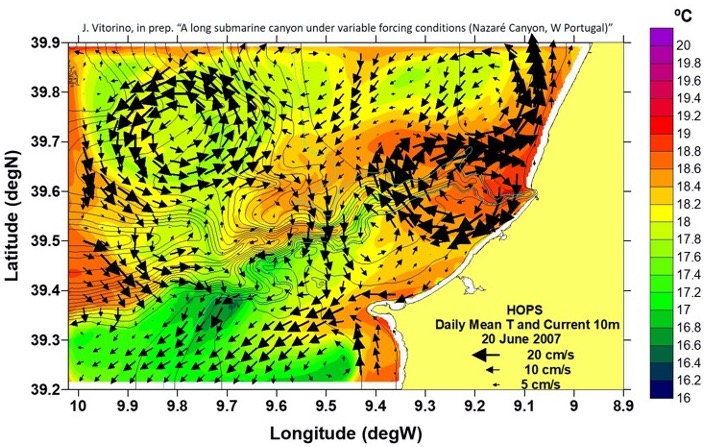
\includegraphics[scale=0.40]{fig/model.jpeg}}
%   \subfigure[MUR SST image for June 20\textsuperscript{th} 2007. The
%   red rectangle covers the area to be modeled in
%   HOPS.]{\label{fig:SST}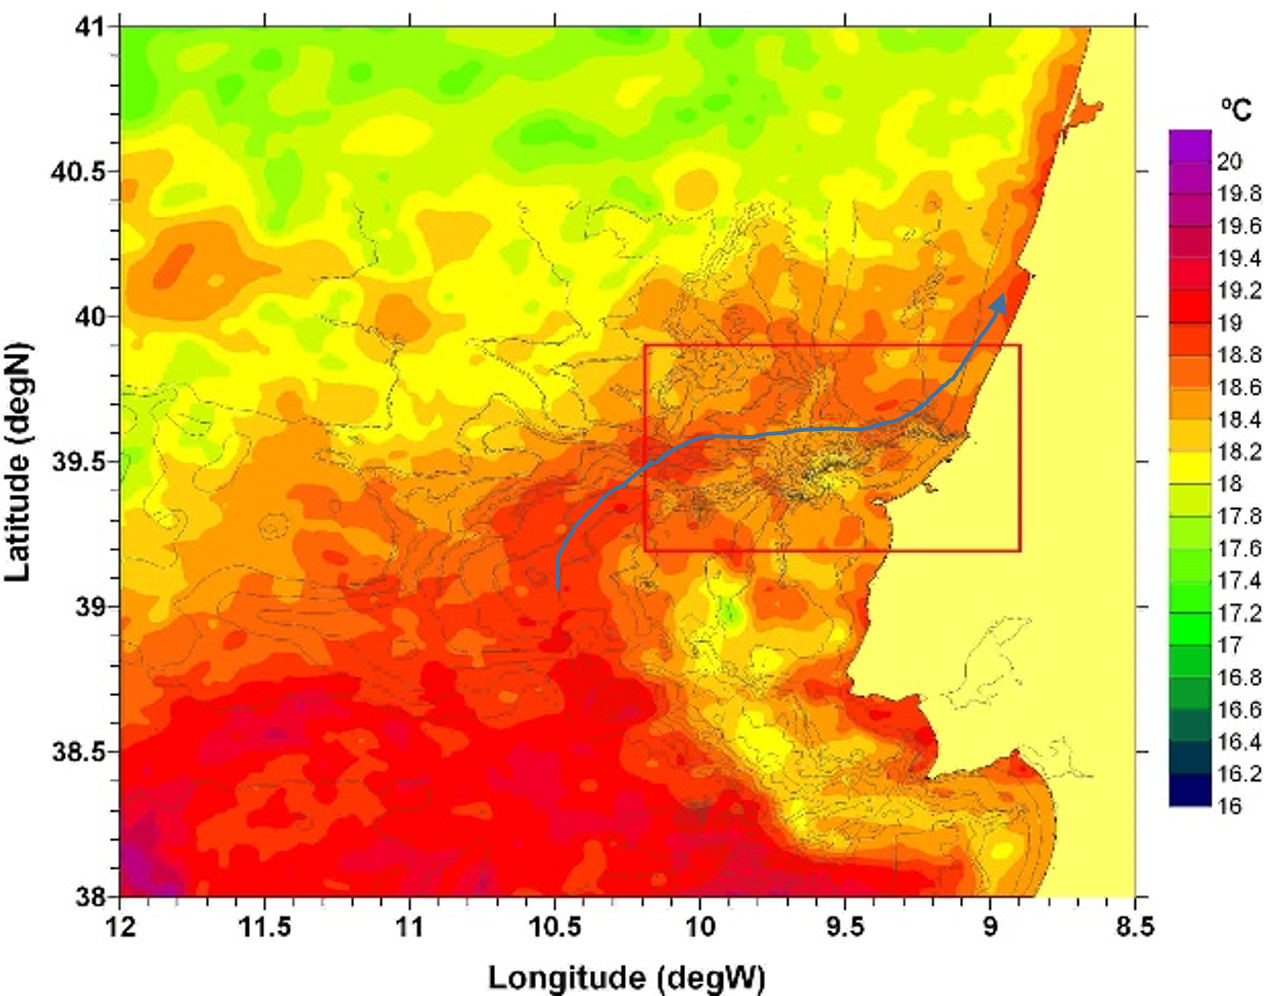
\includegraphics[scale=0.45]{fig/SST-Nazare.png}}
%   \caption{}
% \vspace{-0.5cm}
% \end{wrapfigure}

The geographical domain in which \proj will focus on constitutes a key
area for the shaping of several main characteristics of the
shelf/slope oceanography of the northwestern Portuguese and Spanish
land-mass.  The important changes in the continental margin topography
that characterize this area lead to adjustment processes that impact
not only the local coastal environment but also, in a still poorly
known manner, the wider domain that extends to the north.

% The marked changes in the continental margin topography
% that characterize this area play an important role in establishing the
% nature of the shelf response to wind forcing or the adjustment of the
% poleward slope intensified flow. The area (Fig. \ref{fig:model}) shows
% several expressive examples of coastal mesoscale features such as the
% large upwelling filament of Cabo Carvoeiro which is one of the larger
% and more persistent features of the summer upwelling regime in the
% western portuguese coast, with an expression similar to the large
% filaments off of Cape Finisterre (northwestern Spanish coast), Cape da
% Roca (near Lisbon) or Cape S.Vicente (in the southwestern tip of
% Portugal).

The area hosts important coastal meso-scale features such as the
upwelling filament of Cape Carvoeiro (Penich) that extends for more
than 200 km and is a recurrent feature of the summer upwelling regime
along the western Iberian coast together with the large filaments off
Cape Finisterre in the northwestern Spanish coast, of Cape da Roca in
the area near Lisbon or of Cape S.Vicente in the southwestern tip of
Portugal \cite{haynes93}.

A rich variety of other coastal meso-scale and sub meso-scale
processes are linked to the presence of the Nazare Canyon. Among these,
\proj will focus on processes that:

\begin{itemize}

\item manifest on a relatively small geographical area; this would
  allows us to show the full potential of autonomous platform
  measurements in providing a detailed understanding of the processes

\item impact the local ecosystems; bringing together the physical,
  chemical and biological observations in a systematic manner and
  building a basis to support local fisheries and management of
  protected areas

\item potentially extend their influence to a broader area, shaping
  the conditions observed along the northwestern Portuguese margin; in
  this manner the local observations conducted in \proj will also
  contribute to a better understanding of the conditions prevailing in
  the wider region

\item are relevant for the operational support to navy operations or
  during crises at sea

\end{itemize}  

% The long and narrow \naz Canyon in addition promotes a rich variety of
% coastal mesoscale and submesoscale processes that not only directly
% affect the local ecosystems but can also contribute to impact a much
% larger coastal ocean area. Since they are linked to the canyon
% dynamics these processes develop on a relatively small area of the
% coastal ocean which are associated with specific areas of the canyon
% topography. In this way a strategy that concentrates several
% observation systems in this small area can bring considerable insight
% on the nature of the processes. This concentration is of particular
% interest for \proj objectives. \kc{TO BE CONTINUED...\ldots}
 
Two categories of processes that conform to the above requirements
will be the object of \proje's attention and are described below. The
exact nature of the processes to be covered during the field
experiment will depend on the period of the year during which the
experiment will take place and on the prevailing forcing conditions
that affect the \naz canyon area during the operational window of the
experiment.

\begin{description}
  
\item[Process Category 1] Localized areas of intensified upwelling and
  biological development promoted by the canyon.

  Some important processes relate to the interaction of the shelf and
  slope circulation with the canyon topography during periods of
  favorable upwelling wind forcing. The basic mechanism for the
  response of a narrow canyon to these type of forcing conditions is
  well known -- namely the breakdown of geostrophy when the upwelling
  jet passes over the abrupt canyon topography which promotes an
  up-canyon circulation and with the intensification of upwelling of
  cold, nutrient rich subsurface waters at the canyon head
  \cite{klinck96,she00}. Advection by the upwelling jet, displaces the
  area of upward motion and nutrient intake in the upper layers to the
  leeward flank of the canyon and adjacent shelf allowing this
  influence to affect a large shelf area. In long submarine canyons in
  addition, other processes come into play to prime the persistence of
  upwelling conditions even when forcing decays, leading to a seasonal
  upwelling condition instead of an event-driven response
  \cite{allen00,waterhouse09}.

  The expression of these processes in the \naz canyon is however much
  more complex and depends on the maturity of upwelling
  conditions. During the early stages of the upwelling season or
  during isolated upwelling events in the shelf away from the canyon,
  the response to wind forcing is concentrated in the inner and mid
  shelf. The water source from upwelling comes from relatively shallow
  depths over the shelf below the \emph{Ekman layer} and the upwelling
  conditions are very depended on the variability of the wind forcing
  \kc{being rapidly degrade in favorable wind decay or
    inverse}. During such types of conditions previous observations
  suggest that the response of the \naz canyon was consistent with the
  general mechanism described above, with upwelling of cold and
  nutrient rich waters occurring along the southern flank of the
  canyon and affecting the shelf to the south of the canyon head.
 
  \textsl{Specific Scientific Question 1:} if one of the periods
  described above is covered during the \proj field program we will
  take advantage of the combination of high resolution observations
  and data assimilation models to get unparalleled insight into the
  physical, chemical and biological processes that play together in
  the intensified upwelling at the \naz canyon head. Given the
  position of the canyon head very near the coast, the study will also
  focus the interaction of these processes with the littoral
  environment. In addition, if the period of observation covers an
  upwelling condition that occurs during winter or early
  spring, an associated focus of interest will be to understand the
  impact \kc{of the circulation associated with the canyon in canyon a
  particular attention will be paid to the impacts}
 
A different picture emerges during more mature phases of the upwelling
that develops when favorable winds persist for a few months. This is
typically the case at the end of the summer upwelling season (by
August and September) but can develop earlier in the year if the
previous winter conditions were marked by a positive phase of the
winter NAO (and prevailing upwelling favorable northerly winds). Away
from the canyon, the persistent upwelling favorable forcing builds an
upwelling response that now extends to the complete water column over
the shelf, expressed by an upward lift of isopycnics affecting the
first 200 m depth or more. The source water for upwelling now comes
from depths of 200--300 m over the upper slope. Although the surface
levels respond rapidly to the wind forcing and a decay or inversion of
the upwelling favorable winds can lead to the suppression of upwelling
conditions at near surface depths, this response does not remove the
expression of upwelling below. Consequently with the re-establishment
of the upwelling favorable forcing the mature upwelling conditions are
re-established very rapidly. These are characterized by cold upwelled
waters extending over the complete continental shelf and the upwelling
front and jet being located over the outer shelf/upper slope region.

During those periods, the upwelling jet intersects the \naz canyon
further offshore, primarily in the outer part of the upper canyon
section. The canyon topography and the blocking upwelling of the
topography due to the ridge between Cape Carvoeiro and Berlengas
Islands, both contribute to deflect the upwelling jet towards the
southern flank of the canyon. \kc{Here marked expression of this were
  observed in the physical and biological (fluorometry) fields and}
 
\textsl{Specific Scientific Question 2:} If the \proj field program
takes place during a mature stage of upwelling such as the one
described above we want to understand what processes take place in
this area along the southwestern flank of the upper \naz canyon. In
particular we want to evaluate how these processes are affecting the
marine ecosystems of the Berlengas Archipelago, a marine protected
area.

\item[Process Category 2] Closed circulation cells promoted by the
canyon during wind forcing transitions.

Marked closed circulation cells are observed over the canyon
topography, near the canyon head during periods of decay or inversion
of the wind forcing conditions. These closed circulations are
associated with the inner canyon circulation and vertical motion near
the canyon head that was established in the canyon during periods
of active forcing and that persist after the decay of the forcing
conditions and are no longer advected by the shelf circulation. The
importance of these cells relies on their potential for confinement of
nutrient fluxes, phytoplankton and zooplankton in a relatively small
geographical area, potentially boosting rapid biological development
at all trophic levels.

This importance can be particularly expressive in the closed
circulation cells that are established after a period of active
upwelling, during the phases of weakening or inversion of the
upwelling favorable winds. During the phase of active upwelling the
upward flux of cold nutrient rich subsurface waters that is
promoted at the canyon head is advected southwards by the upwelling
jet, affecting a broad area of the shelf. In contrast, during the
relaxation of upwelling, the upward motion subsists but is no longer
advected, remaining confined to the closed circulation cell over the
canyon. In this case the confinement of nutrient fluxes and biological
species (phytoplankton, zooplankton) can boost a response in terms of
biological development that, although spatially restricted, can be
more significative than during active phases of upwelling.

Closed circulation cells over the canyon are also observed just after
periods dominated by downwelling conditions, when the wind forcing
relaxes or inverts. One potentially important scenario can develop
during the winter and early spring in years dominated by the negative
phases of the winter NAO. During those periods the western Portuguese
coast is affected by the passage of synoptic low pressure systems that
promote important precipitation and lead to rapid and significant
discharges of the small rivers and water courses that indent the
coastline between Peniche and \naze.  If downwelling conditions
persist, the fresh and nutrient rich water plume remains confined near
the coast by the onshore surface transport, extending northwards along
the coast. Instead, if upwelling conditions develop the freshwater
plume is transported offshore (and southward), extending over the
complete shelf as a thin surface layer (about 10 m depth) as shown by
previous observations \kc{citation?}. During the decay phase of wind
forcing the closed circulation cell that develops over the canyon can
contribute to the capture of these waters over the canyon, eventually
even to allow them to extend to deeper levels of the water column by
the downward motion at the canyon head that was associated with the
previous downwelling conditions. \kc{This can}

\textsl{Specific Scientific Question 3:} If the \proj field program
takes place during a period of wind forcing transition, the efforts
will concentrate on these closed circulation cells located over the
canyon near the canyon head, in order to understand how these features
develop and what are the key impacts they have in potentially boosting
biological development at different trophic levels.

Independently of the type of conditions that affect the \naz canyon
area during \proje, it will to provide a solid foundation to answer to
one additional specific question, namely:

\textsl{Specific Scientific Question 4:} What is the impact of
offshore slope circulation on the processes described in Specific
Questions 1, 2 and 3?

As described in Section \ref{sec:naz} the area where the \naz canyon
is inscribed is marked by the complex transition from the large
Estremadura Plateau (south of Peniche) to a relatively narrow shelf
(north of Peniche). This change in the topography has a profound
impact on the expression of slope circulation that enters in this
area. Two main components of the slope circulation are in evidence
here. In the first 300 m depth the slope circulation is forced by the
interaction of the eastward oceanic transport with the continental
slope topography through the JEBAR (Joint Effect of Baroclinicity and
Relief \cite{huthnance84} mechanism. This mechanism forces an
intensified slope circulation -- the Iberian Poleward (Slope) Current
(IP(S)C adapting the designation proposed by Peliz et al, 2000) - that
transports northward warm and saltier water from the region southwest
of the Iberian Peninsula along the western continental margin of
Portugal and Spain. While the surface expression of this slope
current, in the upper 100 m depth, can be modulated by wind forcing,
while being reinforced during periods of southerly winds and
downwelling and being suppressed and inverted during periods of
northerly winds and upwelling, the subsurface expression is maintained
as a poleward slope undercurrent that influences depths between 100 m
and 300 m. \kc{The}

\end{description}  